\section{Numerical results}
\subsection{Bar test case}
\subsubsection{Description}
The bar test case is composed of two parts and it is mainly summarized by the figure \ref{fig:bar}. 
\begin{figure}[H]
  \centering
  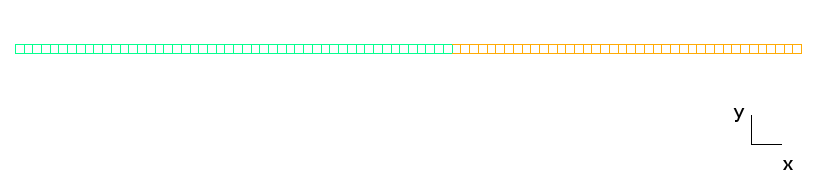
\includegraphics[scale=0.6]{images/bar.png}
  \caption{bar with the medium (left) and the PML (right)}
  \label{fig:bar}
\end{figure}  
This test case corresponds to a simple bar with on the left an elastic medium of a length of $250$ and on the right a PML with a length of $200$. The size of an element is $5$, thus the elastic medium contains $50$ elements whereas the PML $40$. The parameters of the medium are the following and they are the same for the PML.
\begin{table}[H]
\centering
\begin{tabular}{c|c}
$\nu$ & $0.24$ \\
$E$ & $1e07$ \\
$\rho$ & $1700$ \\
\end{tabular}
\end{table} 
In order to calculate the coefficients of attenuation $a_0$ (for propagating waves) and $b_0$ (for evanescent waves) in both directions, we will use the formulation \ref{eq:alpha_kucu} with the reflection wanted at the end of the PML $R_{pp} = 1e-3$. The order of the attenuation functions is $n = 2$. \\
\subsubsection{Non-harmonic input wave}
In the context of the analysis of sismic data, the Ricker wave is often used. It is the normalized negative of the second derivative of a Gaussian function and takes the formulation at the point $x$ ant time $t$:
\begin{equation}
F(x,t) = A \left(2 \pi^2 \frac{(t-t_s)}{t_p^2} -1\right) \exp\left(-\pi^2 \frac{(t-t_s)}{t_p^2}\right)
\end{equation}   
With $t_s$ the time shift, $t_p$ the fundamental period and $A$ the amplitude.
In term of displacement this wave has the following "mexican hat" form:
\begin{figure}[H]
  \centering
  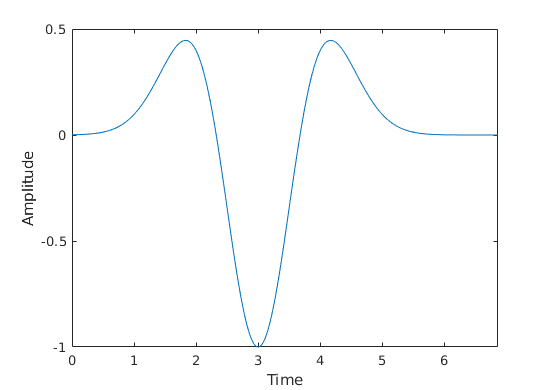
\includegraphics[scale=0.8]{images/ricker.png}
  \caption{Ricker wave in time domain}
  \label{fig:Ricker}
\end{figure}  
We will inject this wave at the left extremity of the medium and fix its propagation within the $x$ direction. We will choose the set of parameter $t_p = 3$, $t_s = 3$ and $A = 1$ which gives us exactly the wave shown in figure \ref{fig:Ricker}.
\subsubsection{Analysis of the results}
We will use the Implicit Newmark scheme as integration scheme. The analysis of the performance will not be reviewed since it is a very simple test case. Therefore a comparison between the results obtained with the Explicit scheme is not needed. Both scheme are able to be accurate and performant on a simple case like the bar test. For more complex case, it will be interresting to compare the scheme and highlights the pros and cons of both schele. For our analysis, a specific attention will be dedicated to the reflexion of the wave due to the interface. The time step used is $dt = 0.025$. For this test case the critical time step is $0.06$.\\ 

Let us record the displacement of a node placed at the center of the elastic medium in both directions. 
\begin{figure}[H]
\centering
\begin{minipage}{.5\textwidth}
  \centering
  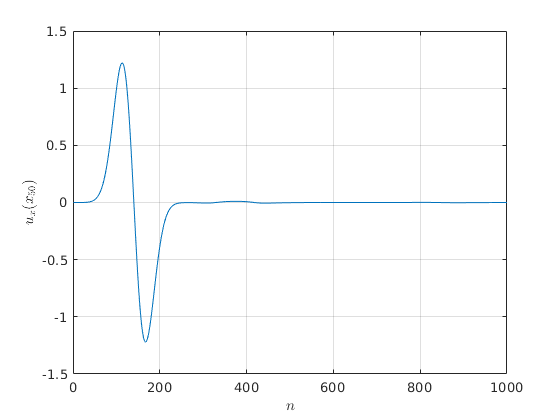
\includegraphics[width=1.\linewidth]{images/disp_imp_x.png}
\end{minipage}%
\begin{minipage}{.5\textwidth}
  \centering
  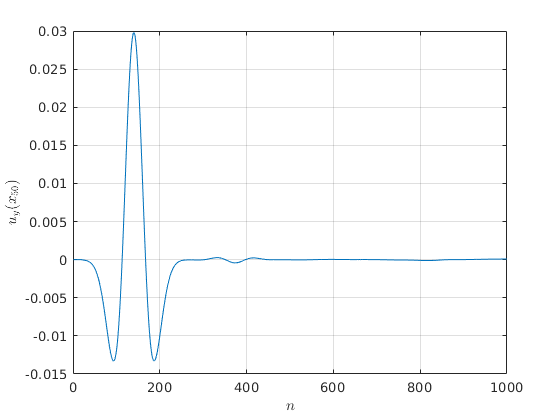
\includegraphics[width=1.\linewidth]{images/disp_imp_y.png}
\end{minipage}
\caption{Displacement within the $x$ direction (left) and $y$ direction (right)}
\label{fig:disp_imp_pml}
\end{figure} 
To understand the results shown on the figure \ref{fig:disp_imp_pml}, an explanation step by step of what is happening is necessary:
\begin{itemize}
\item \underline{Time steps: $[0-300]$} The node records the displacement due to the propagation of the wave in the elastic medium.  
\item \underline{Time steps: $[300-500]$} A very slight reflection can be observed due to the truncation interface. The node records this very small displacement because the reflected wave comes back toward the elastic medium. This wave will bounce back at the left extremity of the medium and will propagate again in direction of the PML.
\item \underline{Time steps: $[500-1000]$} The reflected wave encounters the truncation interface. On this figure the reflection at the point is negligeable and we can consider that the wave is fully attenuated. 
\end{itemize}
Of course this reflexion due to the truncation interface is a key element of the simulation since the perfectly matched layer is designed to be able to minimize it. A simple ratio between the maximum of the initially propagated wave and the reflected one gives $0.0081$. Therefore less than $1\%$ of the wave is reflected by the interface.
Of course taking a smaller value of time step and size of element will decrease this coefficient of reflected wave. We have seen in the stability analysis that the implicit scheme commits an error that evolves with the time step considered.\\
The analysis of the energy of the system is important since the PML has the faculty of attenuate wave, it has also the power of decaying the energies in the system.
\begin{figure}[H]
  \centering
  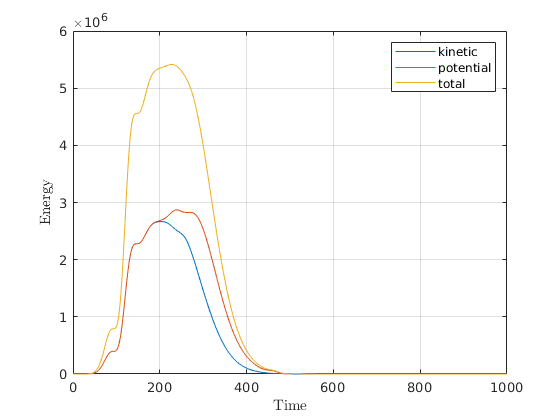
\includegraphics[scale=0.8]{images/simple_test_energies_imp.png}
  \caption{Potential, kinetic and total energies}
  \label{fig:simple_test_en_imp}
\end{figure}          
The energies starts growing together as the wave enters the medium. Once the wave reaches the PML, the energies start decaying rapidly and reaches a value close to $0$. In fact a close analysis of the figure \ref{fig:simple_test_en_imp} and zooming on it, we can conclude that the energies tend to $0$. 

\subsection{Lamb's test case}
The Lamb's test consists in an infinite half space medium and the application of a load, given by a Ricker wave, at the surface. This context can be summarized by the figure \ref{fig:Lamb_test}. The left size disposes of symmetry conditions and the medium is surrounded on the left size and in the depth by a PML. This situation permits to simulate the propagation of sismic waves. The simulation will involves P-, S- and Rayleigh waves which are key waves in the analysis of sismic scenarios.      